\documentclass[11pt]{article}

% Document settings, taken from Introduction to Algorithms (Dinitz).
\usepackage{epsfig}
\usepackage{amsfonts}
\usepackage{amssymb}
\usepackage{amstext}
\usepackage{amsmath}
\usepackage{xspace}
\usepackage{hyperref}
\usepackage{fullpage}
\usepackage{enumitem}                     
\usepackage{titlesec}
\usepackage{amsthm}

\titleformat*{\section}{\bfseries}
\titleformat*{\subsection}{\bfseries}
\titleformat*{\subsubsection}{\bfseries}
\titleformat*{\paragraph}{\bfseries}
\titleformat*{\subparagraph}{\bfseries}

\newcommand{\R}{\ensuremath{\mathbb R}}
\newcommand{\C}{\ensuremath{\mathbb C}}
\newcommand{\N}{\ensuremath{\mathbb N}}
\newcommand{\F}{\ensuremath{\mathbb F}}
\newcommand{\e}{\epsilon}
\newcommand{\E}{\exists}
\newcommand{\sse}{\subseteq}
\newcommand{\union}{\cup}
\newcommand{\meet}{\wedge}
\newcommand{\ra}{\rightarrow}
\newcommand{\ceil}[1]{\ensuremath{\left\lceil#1\right\rceil}}
\newcommand{\floor}[1]{\ensuremath{\left\lfloor#1\right\rfloor}}

\theoremstyle{plain}
\newtheorem{thm}{Theorem}[section]
\newtheorem{lem}{Lemma}[section]
\newtheorem{prop}{Proposition}[section]
\newtheorem{coro}{Corollary}[section]
\newtheorem{obs}{Observation}[section]

\theoremstyle{definition}
\newtheorem{defi}{Definition}[section]

\theoremstyle{remark}
\newtheorem{exm}{Example}[section]
\newtheorem{exc}{Exercise}[section]
\newtheorem{rem}{Remark}
\newtheorem{question}{Question}
\newtheorem{answer}{Answer}

\setenumerate[0]{label=(\alph*)}


%%%%%%%%%%%%%%%%%%%%%%%%%%%%%%%%%%%%%%%%%%%%%%%%%%%%%%%%%%%%%%%%%%%%%%%%%%%
%%%%%%%%%%%%%%%%%%%%%%%%%% Document begins here %%%%%%%%%%%%%%%%%%%%%%%%%%%
%%%%%%%%%%%%%%%%%%%%%%%%%%%%%%%%%%%%%%%%%%%%%%%%%%%%%%%%%%%%%%%%%%%%%%%%%%%


\begin{document}

% EDIT THE FOLLOWING PARAMETERS FOR EACH ASSIGNMENT.

% NAME and COURSE TITLE + SECTION NUMBER
\noindent {\large {\bf Matrix Analysis and Linear Algebra}} \hfill {\bf Dr. Donniell Fishkind}

% PROFESSOR and HOMEWORK NUMBER
\noindent {{\bf TA: } Ronak Mehta} \hfill 
{Discussion Section Notes}

\noindent \rule[0.1in]{\textwidth}{0.4pt}

% CONTENT

\section{September 3, 2019}

\subsection{Section format}
\begin{itemize}
    \item Go over old homework solutions.
    \item Reiterate concepts from class.
    \item (Optional) Make connections to ideas from statistics or optimization.
    \item Answer any questions that you have.
\end{itemize}
{\bf Note:} I will prepare material for each section, but your questions are universally more important than whatever I prepare, so please ask them.
\subsection{Algorithm for success}
\begin{enumerate}
    \item Attend every class.
    \item Take exhaustive notes, typeset them in real-time or otherwise.
    \item View homework immediately after posting.
    \item Memorize lecture notes verbatim prior to exams.
\end{enumerate}

\subsection{Real analysis review}

\begin{defi}[Metric space]
    Let $X$ be a set. Let $d: X \times X \ra [0, \infty)$ with the following properties.
    \begin{enumerate}
        \item $d(x,y) \geq 0$ and $d(x,y) = 0 \iff x = y$ for $x, y \in X$. (Identity of indiscernables)
        \item $d(x,y) = d(y, x)$ (Symmetry)
        \item $d(x,y) \leq d(x,z) + d(z,y)$ for $x, y, z \in X$. (Triangle inequality)
    \end{enumerate}
    The tuple $(X, d)$ is called a metric space.
\end{defi}

\begin{exm}
    $X = \R$ and $d(x,y) = |x - y|$
\end{exm}
\begin{exm}
    $X = \R^n$ and $d(x,y) = ||x - y||_2 = \sqrt{\sum_{i=1}^n (x_i - y_i)^2}$, the Euclidean distance.
\end{exm}

\begin{defi}[Sequence]
    A sequence $(x_n)_{n=1}^\infty = x_1, x_2,...$ is a countably infinitely long list.
\end{defi}

\begin{defi}[Limit of a sequence]
    A sequence $(x_n)_{n=1}^\infty$, where $x_n \in (X,d)$, converges to limit $x \in (X,d)$ if $\forall \e > 0, \E N(\e):$
    \begin{align*}
        \forall n \geq N, \ d(x_n, x) < \e
    \end{align*}
\end{defi}
Note that convergence requires the limit to be in the space.
\begin{exm}
    The sequence $3, 3.1, 3.14, 3.141$ approaches $\pi$, but if our metric space was restricted to just the rational numbers $\mathbb{Q}$, then we would not call this a convergent sequence.
\end{exm}
\begin{exm}
    Let $x_n = \frac{1}{n}$. This sequence has limit $x = 0$.
    \begin{proof}
    Given any $\e$, let $N = \ceil{\frac{1}{\e}}$. Then, for $n \geq N:$
    \begin{align*}
        d(x_n, x) &= \left|\frac{1}{n} - 0\right| = \frac{1}{n} \leq \frac{1}{N} \leq \frac{1}{\tfrac{1}{\e}} = \epsilon
    \end{align*}
    \end{proof}
\end{exm}
\begin{defi}[Cauchy sequence]
    A sequence $(x_n)_{n=1}^\infty$, where $x_n \in (X,d)$, is Cauchy if $\forall \e > 0, \E N(\e):$
    \begin{align*}
        \forall k,l \geq N, \ d(x_k, x_l) < \e
    \end{align*}
\end{defi}
\begin{exm}
    The sequence $x_n = \frac{1}{n}$ is Cauchy. 
    \begin{proof}
    Given any $\e$, let $N = \ceil{\frac{2}{\e}}$. Then, for $k,l \geq N:$
    \begin{align*}
        d(x_k, x_l) &= \left|\frac{1}{k} - \frac{1}{l}\right| \leq \frac{1}{k} + \frac{1}{l} \leq \frac{2}{N} \leq \frac{2}{\tfrac{2}{\e}} = \epsilon
    \end{align*}
    \end{proof}
\end{exm}
\begin{figure}
    \centering
    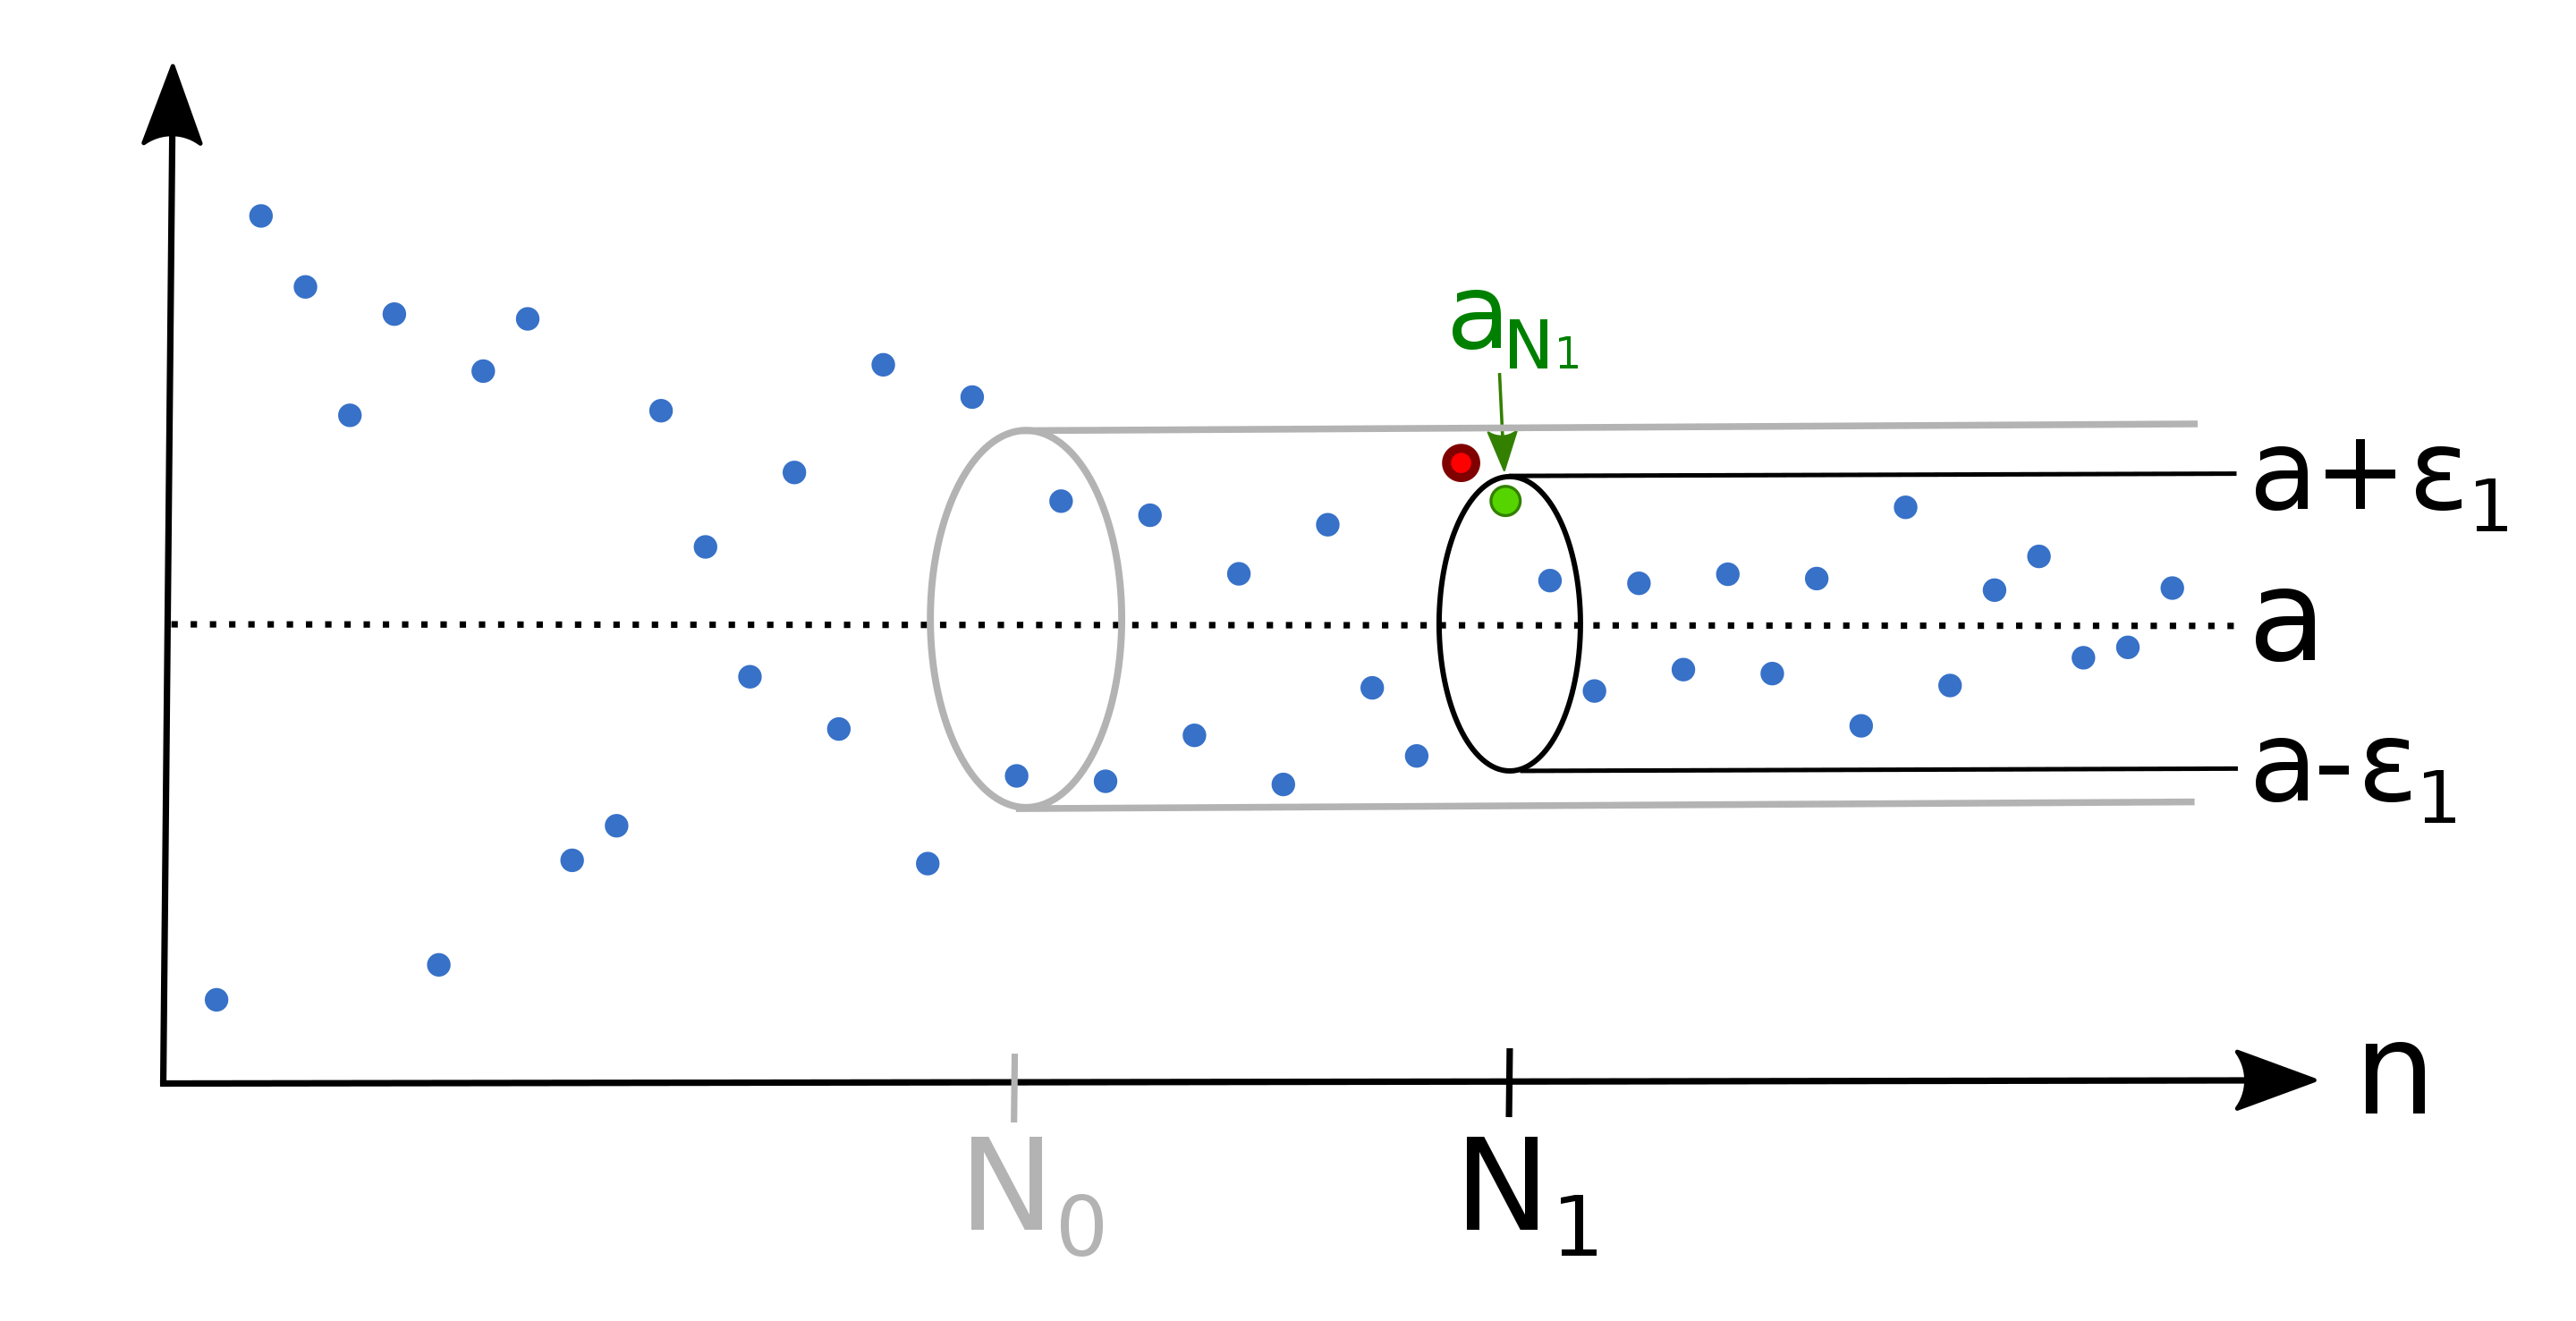
\includegraphics[width=\linewidth]{figures/limit.png}
    \caption{$a$ denotes the limit in this sequence, $N_0$ denotes $N(\epsilon_0)$ for some $\epsilon_0$, and $N_1 = N(\epsilon_1) < N_0$ for some $\epsilon_1 < \epsilon_0$.}
\end{figure}
\begin{exc}
    Prove that a sequence converges $\implies$ the sequence is Cauchy.
\end{exc}
\begin{defi}
    A metric space $(X,d)$ is complete if every Cauchy sequence converges.
\end{defi}

\begin{defi}[Open ball]
    An open $\e$-ball about $c$ is the set $B_{\e}(c) = \{x : d(x,c) < \e\}$.
\end{defi}
\begin{defi}[Accumulation point]
    Let $A \sse X$. Point $a$ is an accumulation point of $A$ if 
    \begin{align*}
        \forall \e > 0 \ \E x \in A: x \neq a \text{ and } x \in B_{\e}(a)
    \end{align*}
    In other words, every open $\e$-ball about $a$ contains a point from $A$ that is different from $a$.
\end{defi}
\begin{exm}
    Let $X = \R$. The set $A = [0, 1)$ has accumulation point 1, as every interval $B_{\e}(1) = (1 - \e, e + \e)$ contains a point in $[0,1)$.
\end{exm}
\begin{defi}[Open set]
    A set $A \sse X$ is called open if for every $x \in A$, $\E \e>0 : B_{\e}(x) \sse A$. In other words, for every point in $A$, a small enough open ball about that point is also in $A$.
\end{defi}
\begin{exm}
    Let $X = \R$. The set $A = (0, 1)$ open.
    \begin{proof}
    Formally, let $x \in (0,1)$. Let $\e = \min\{x, 1-x\}$. Then, $B_{\e}(x) \sse (0,1)$.
    \end{proof}
\end{exm}
\begin{exm}
    Any open ball is open.
    \begin{proof}
    Using the notation from the figure below, let $A = B_r(x)$ be an open ball in $(X,d)$. Choose $y \in A$. Let $\e = r - d(x,y)$. To show that $B_{\e}(y) \sse B_r(x)$, take any point $z \in B_{\e}(y)$. By construction, we have:
    \begin{align*}
        d(y, z) < \e = r - d(x,y) \implies d(y, z) + d(x, y) < r
    \end{align*}
    To show that $z \in B_r(x)$, we bound $d(x,z)$ by $r$.
    \begin{align*}
        d(x,z) \leq d(y, z) + d(x, y) < r
    \end{align*}
    \end{proof}
\end{exm}
\clearpage
\begin{figure}
    \centering
    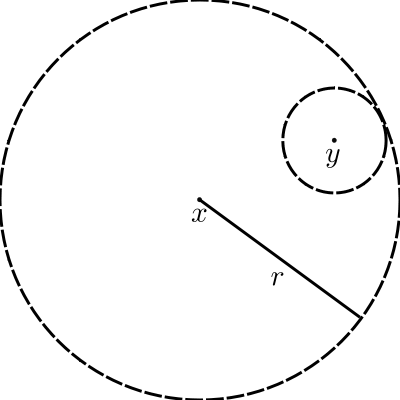
\includegraphics[width=0.5\linewidth]{figures/open_ball.png}
    \caption{An open $r$-ball about $x$. Dotted lines typically denote the unincluded boundary of the set.}
\end{figure}
\begin{defi}[Closed set]
    A set $A$ is closed if it contains all of its accumulation points.
\end{defi}
\begin{exm}
    As seen above, $[0,1)$ has (only) accumulation point 1. Thus the set $[0,1]$ is closed.
\end{exm}
\begin{thm}
    $A$ is open if and only if $A^c$ is closed.
\end{thm}
\begin{rem}
    In $\R$, the sets $\R$ and $\emptyset = \{\}$ are both open and closed.
\end{rem}
\begin{rem}
    A finite set $A = \{x_1, x_1, ..., x_n\}$ is closed. With distinct elements, no point is an accumulation point, thus all are contained.
\end{rem}
\begin{thm}
    The following hold in $(X,d)$.
    \begin{enumerate}
        \item An arbitrary number of unions of open sets is open.
        \item A finite number of intersections of open sets is open.
        \item A finite number of unions of closed sets is closed.
        \item An arbitrary number of intersections of closed sets is closed.
    \end{enumerate}
\end{thm}
\begin{exm}
    Let $A_n = (-\frac{1}{n}, \frac{1}{n})$. Each $A_n$ is open. However, $A = \bigcap_{n=1}^\infty A_n = \{0\}$ which is not open.
\end{exm}
\begin{exm}
    Let $A_n = \{\frac{1}{n}\}$. Each $A_n$ is closed. However, $A = \bigcup_{n=1}^\infty A_n = \{\frac{1}{n} : n = 1, 2, ..\}$, which has accumulation point 0, and is thus not closed. 
\end{exm}

\section{September 10, 2019}

\subsection{Real analysis review, cont'd}

\begin{defi}[Open cover]
    An open cover of set $A$ is a (possibly infinite) collection of open sets $\mathcal{S}$ such that $A \sse \bigcup_{O \in \mathcal{S}} O$. A subcover is a subset of $\mathcal{S}$ that is still a cover for $A$
\end{defi}
\begin{defi}[Compact set]
    The following are equivalent statements.
    \begin{enumerate}
        \item A set $A$ is compact.
        \item Every open cover of $A$ has a finite subcover.
        \item Every sequence $x_1, x_2,...$ with $x_n \in A$ has subsequence that converges to $x \in A$.
    \end{enumerate}
\end{defi}
\clearpage
\begin{figure}
    \centering
    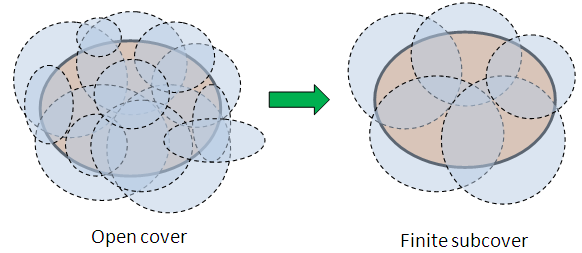
\includegraphics[width=0.8\linewidth]{figures/finite_subcover.png}
    \caption{The brown ellipse represents a set, and the blue ellipses represent an open cover. Note that compactness does not require the existence of an open cover, but for every given (even infinite) open cover, one can extract a finite subcover.}
\end{figure}
These definitions can be difficult to verify. In $\R^n$, there is a simpler characterization.
\begin{defi}[Boundedness]
    A set $A$ is bounded if there exists a point $c \in X$ with finite radius $r$ such that $A \sse B_r(c)$. In other words, $A$ is bounded if an open ball can contain it fully.
\end{defi}
\begin{thm}[Heine-Borel]
    $A \in \R^n$ is compact if and only if it is closed and bounded.
\end{thm}
\clearpage
\begin{figure}
    \centering
    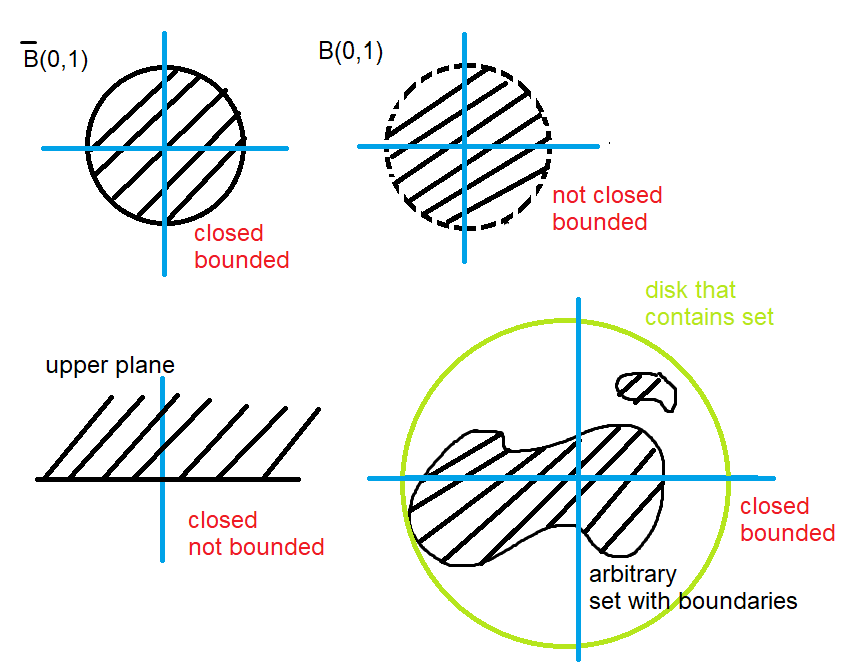
\includegraphics[width=\linewidth]{figures/compact.png}
    \caption{The shaded regions represent elements of the set, with solid and dotted boundaries denoting inclusion and exclusion, respectively. The top-left and bottom-right are compact sets in $\R^2$.}
\end{figure}
\begin{exm}
    In $\R$, a closed interval $[a, b]$ is compact.
\end{exm}
\begin{exm}
    In $\R^n$, the unit sphere $A = \{x : ||x||_2 = 1\}$ is compact (where $||x||_2 = \sqrt{\sum_{i=1}^n x_i^2}$).
\end{exm}
\begin{defi}[Continuity]
    Let $f: (X, d_X) \rightarrow (Y, d_Y)$. $f$ is continuous at $x_0$ if for every $\e > 0$, there is a $\delta(\e, x_0)$ such that $\forall x \in X$:
    \begin{align*}
        d(x, x_0) < \delta \implies d(f(x), f(x_0)) < \e
    \end{align*}
    $f$ is continuous if it is continuous at all $x_0 \in X$.
\end{defi}
The definition of continuity captures the notion that small changes in $x$ should result in small changes in $f(x)$. Specifically, the change in $f(x)$ should be made arbitrarily small by controlling the change in $x$. Note that $\delta$ depends on both $\e$ and $x_0$. 
\clearpage
\begin{figure}
    \centering
    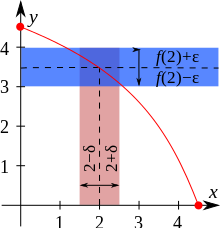
\includegraphics[width=0.5\linewidth]{figures/continuous.png}
    \caption{This function is continuous at $x = 2$.}
\end{figure}
\begin{defi}[Uniform continuity]
    Let $f: (X, d_X) \rightarrow (Y, d_Y)$. $f$ is uniformly continuous if for every $\e > 0$, there is a $\delta(\e)$ such that $\forall x_0, x_1 \in X$:
    \begin{align*}
        d(x_0, x_1) < \delta \implies d(f(x_0), f(x_1)) < \e
    \end{align*}
\end{defi}
Note that the dependence of $\delta$ on the point in $X$ is not gone.
\clearpage
\begin{figure}
    \centering
    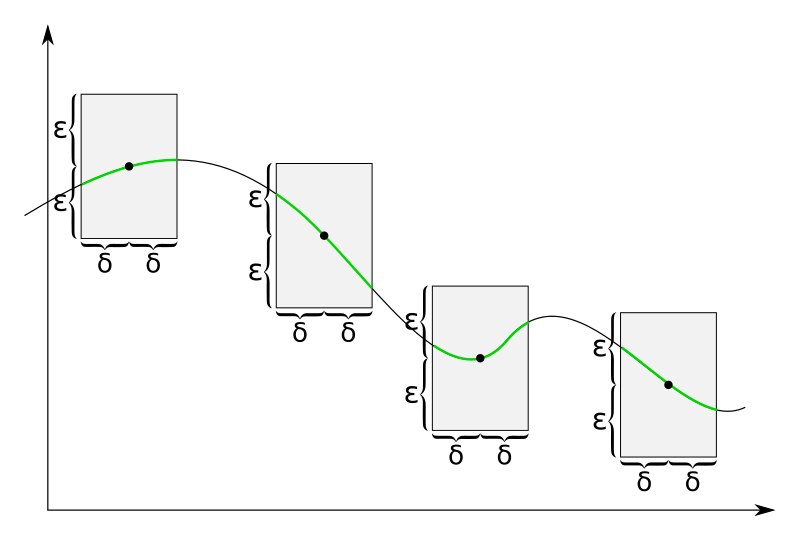
\includegraphics[width=0.494\linewidth]{figures/uniform.png}
    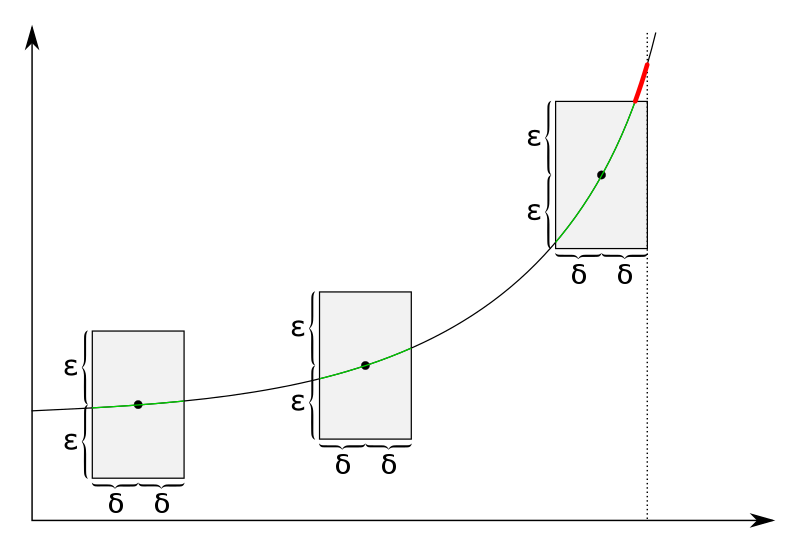
\includegraphics[width=0.494\linewidth]{figures/not_uniform.png}
    \caption{A pictorial characterization of continuity whether a ring of height $2\e$ and width $2\delta$ could slide along the entire function, without turning, for every $\e$. If $\delta$ must change as this happens, the the function is only continuous. In the right example, $\delta$ must get smaller as $x$ gets large in order for the ring to continue sliding. In the case that $\delta$ can stay constant, as in the left example, then the function is uniformly continuous.}
    \label{fig:cont}
\end{figure}

\section{September 17, 2019}

In response to questions from last time:
\begin{exc}
    Show that compactness implies closure in a metric space.
\end{exc}
\begin{exm}
    Show that compactness implies boundedness in a metric space.
    \begin{proof}
        Let $(X,d)$ be the metrix space, and $A$ be the compact set of interest. Chose any $x_0 \in X$, and write $\mathcal{S} = \{B_r(x_0) : r > 0\}$. Clearly, $A \subset \mathcal{S}$, and $\mathcal{S}$ is an open cover of $A$. Thus, there exists a finite subcover
        \begin{align*}
            F = \{B_{r_1}(x_0), ..., B_{r_p}(x_0)\}
        \end{align*}
        Take $r = \max_{i=1,...,p} r_i$, and $A \sse B_r(x_0)$.
    \end{proof}
\end{exm}
\begin{exc}
    Given an example of a metric space that is closed and bounded, but not compact. Hint: Use the discrete metric. That is,
    \begin{align*}
        d(x,y) = \begin{cases}
        0 \text{ if } x = y\\
        1 \text{ if } x \neq y
        \end{cases}
    \end{align*}
\end{exc}
\begin{exm}
    Prove that $f(x) = \frac{1}{x}$ on $x > 0$ is not uniformly continuous.
    \begin{proof}
        Let $\e = 1$. For any $\delta$, we must choose $x_0$ and $x_1$ such that $|x_0 - x_1| < \delta$ does imply that $|f(x_0) - f(x_1)| < 1$.
        \begin{align*}
            |f(x_0) - f(x_1)| = \frac{\delta}{x_0 x_1}
        \end{align*}
        Letting $x_1 = x_0 + \frac{\delta}{2}$.
        \begin{align*}
            |f(x_0) - f(x_1)| = \frac{\delta}{x_0 (x_0 + \frac{\delta}{2})}
        \end{align*}
        Choosing $x_0$ small enough can make this quantity larger than $\e = 1$.
    \end{proof}
\end{exm}

Continuing with the review, there are many useful properties that result from a continuous function on a compact set.
\begin{thm}
    Let $f: (X,d_X) \rightarrow (\R, d_Y)$ be continuous over compact set $X$. Then:
    \begin{enumerate}
        \item $f$ is uniformly continuous.
        \item $f(X) = \{f(x) : x \in X\}$ is compact. 
        \item $f$ achieves $\max_{x \in X} \{f(x)\}$ and $\min_{x \in X} \{f(x)\}$, as in there exists $x^*_{\text{max}}, x^*_{\text{min}} \in X$ such that
        \begin{align*}
            f(x^*_{\text{min}}) \leq f(x) \leq f(x^*_{\text{max}})
        \end{align*}
        for all $x$.
        \item Let $\lim_{n \rightarrow \infty} x_n = x$, where $x_n, x \in X$. Then
        \begin{align*}
            \lim_{n \rightarrow \infty} f(x_n) = f\left(\lim_{n \rightarrow \infty} x_n\right) = f(x)
        \end{align*}
    \end{enumerate}
\end{thm}
\begin{exm}
    Let $f: (X,d_X) \rightarrow (Y, d_Y)$ and $g: (Y,d_Y) \rightarrow (Z, d_Z)$ both be continuous functions. Show that the composition $f \circ g$ is continuous.
    \begin{proof}
        Given any $x_0 \in X$ and any $\e > 0$, let $y_0 = f(x_0)$. Choose $\delta_g(\e, y_0)$ such that:
        \begin{align*}
            d_Y(y_0,y) < \delta_g \implies d_Z(g(y_0), g(y)) < \e
        \end{align*}
        Then choose $\delta_f(\delta_g, x_0)$ such that:
        \begin{align*}
            d_X(x_0,x) < \delta_f \implies d_Y(f(x_0),f(x)) < \delta_g
        \end{align*}
        Thus
        \begin{align*}
             d_X(x_0,x) < \delta_f \implies d_Y(f(x_0),f(x)) < \delta_g \implies d_Z(g(f(x_0)), g(f(x))) < \e
        \end{align*}
    \end{proof}
\end{exm}
\begin{exc}
    Give a function that is bounded, i.e. there is some $B \geq 0$ such that $|f(x)| \leq B$ for all $x \in X$, and continuous, but not uniformly continuous.
\end{exc}
\begin{defi}[Lipshitz continuity]
    A function $f: (X,d_X) \rightarrow (Y, d_Y)$ is called Lipshitz continuous with Lipshitz constant $L$ for all $x_0, x_1 \in X$:
    \begin{align*}
        d_Y(f(x_0), f(x_1)) \leq L \cdot d_X(x_0, x_1)
    \end{align*}
\end{defi}
This means that the changes in $f(x)$ are sublinear in the changes in $x$. The constant $L$ ``quantifies" the continuity of $f$. 
\begin{obs}
    Lipshitz continuity implies uniform continuity.
    \begin{proof}
        Given any $e > 0$, let $\delta = \frac{\e}{L}$.
        \begin{align*}
            d_Y(f(x_0), f(x_1)) \leq L \cdot d_X(x_0, x_1) \leq L \cdot \frac{\e}{L} = \e
        \end{align*}
    \end{proof}
\end{obs}

Pointers for Homework 1:
\begin{enumerate}
        \item Similarity implies sameness of rank, spectrum/charactaristic polynomial and determinant. None of the reverse implications hold.
        \item Same eigenvectors does not imply similarity. What does it imply (assuming there are $n$ of them that are linearly independent)?
        \item What can you say about a matrix with distinct eigenvalues?
        \item What can you say about the eigenvalues of diagonal/triangular matrix?
        \item A matrix is invertible - what can you say about its eigenvalues?
    \end{enumerate}

\section{September 24, 2019}

{\it Homework 1 solutions.}

\section{October 1, 2019}

{\it Homework 2 solutions.}

\section{October 8, 2019}

{\it Copies of Homework 3 solutions distributed.}\\

When I say "application", I mean that these topics are not tested in the course, but topics mostly from mathematical data science that are interesting and make use of material from the course.

\subsection*{Application: Projection Matrices} 

$A^2 = A \in M_n(\R)$. What can you say about this matrix? Given the additional information that $A = A^T$, what else can be said?

The matrix has annihilating polynomial $p(t) = t(t-1)$, therefore any eigenvalues $\lambda \in \{0,1\}$. $q_A$ divides this polynomial, so $q_A$ is the product of distinct linear factors, implying that $A$ is diagonalizable. In fact $Ax = SDS^{-1}x$ is a projection of $x$ onto the subspace spanned by the eigenvectors of $A$ associated with eigenvalue 1. This happens in three steps.
\begin{enumerate}
    \item $y_1 = S^{-1}x$ gives the coordinates of $x$ in the basis described by the columns of $A$.
    \item $y_2 = Dy_1$ scales the components by 0 or 1, eliminating certain dimensions and keeping other.
    \item $y_3 = Sy_2$ brings us back into the original basis.
\end{enumerate}
If $A = A^T$, then it is real orthogonally diagonalizable, with the eigenvectors forming an orthonormal basis. This idea is depicted in Figure \ref{fig:proj}. The transformation $A$ is called a projection matrix. The next topic will make use of ideas from Chapters 0 through 4.

\begin{figure}[h!]
    \centering
    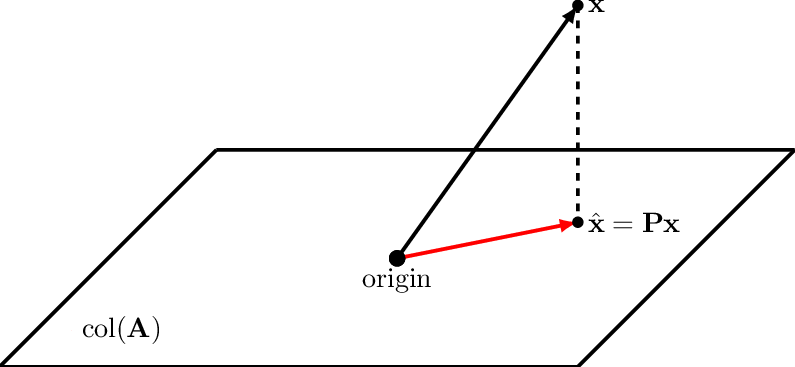
\includegraphics[width=0.6\linewidth]{figures/projection.png}
    \caption{Here ${\bf x} \in \R^3$ is the vector of interest and ${\bf P} \in M_3(\R)$ is the projection matrix. If we ${\bf P} = SDS^{-1}$ let ${\bf A}$ be the $M_{3,2}(\R)$ matrix that column binds the eigenvectors of ${\bf P}$ associated to eigenvalue 1, then the subspace column space of ${\bf A}$.}
    \label{fig:proj}
\end{figure}

\subsection*{Application: Unconstrained Optimization}

Let $f: \R^d \rightarrow \R$ be a twice-differentiable function, with
\begin{align*}
    \nabla f(x) &=: g(x) \in \R^d\\
    \nabla^2 f(x) &=: H(x) \in M_d(\R)
\end{align*}
\begin{defi}[Local minimum]
    $x^*$ is a local minimum of $f$ if there exists an $\e > 0$ such that for all $x \in B_{\e}(x)$, $f(x^*) \leq f(x)$.
\end{defi}

Our goal is to find such a local minimum, and we write this problem as
\begin{align*}
    \min_{x \in \R^d} f(x)
\end{align*}

There are many ways to go about this, but one such was is to iteratively propose candidate solutions $x_1, x_2, ...$ that get ``closer" to a local minimum $x^*$. A subset of these methods is line-search methods, where at iterate $x_t$, we choose a search direction $p \in \R^d$ and step size $\alpha \in [0, 1)$, and let $x_{t+1} = x_t + \alpha p$. For example, in gradient descent, we let $p = - g(x_t)$, as in Figure \ref{fig:grad}.
\begin{figure}[h!]
    \centering
    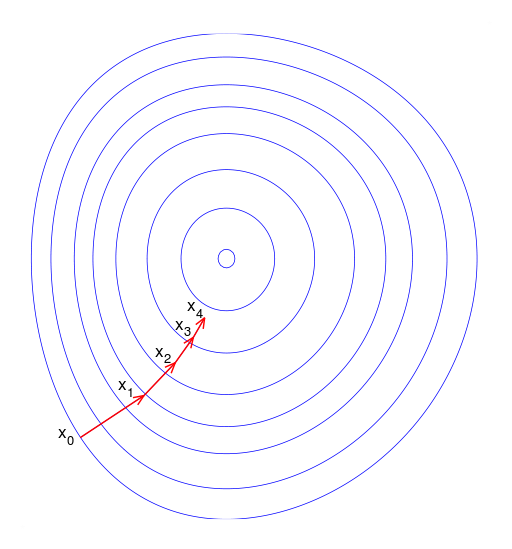
\includegraphics[width=0.5\linewidth]{figures/grad.png}
    \caption{The center of the contour plot is the local minimum.}
    \label{fig:grad}
\end{figure}

Some basic optimality conditions:
\begin{align*}
    \text{$x^*$ is a local minimum.} &\implies g(x^*) = 0 \text{ and  $H(x)$ is P.S.D.}\\
    g(x^*) = 0\text{ and  $H(x)$ is P.D.} &\implies \text{$x^*$ is a local minimum.}
\end{align*}
While we will not prove them, we will attempt to understand them via the Hessian matrix $H(x^*)$. Taylor expand $f(x_0 + \alpha p)$ about $x_0$.
\begin{align*}
    f(x_0 + \alpha p) = f(x_0) + \alpha g(x_0)^T p + \frac{1}{2} \alpha^2 p^T H(x_0) p + o(\alpha^2)
\end{align*}
Assume that we are at a stationary point $x_0$, i.e. $g(x_0) = 0$. Note that $H = H^T$ for any $x$, thus $H$ is real orthogonally diagonalizable. Let $u_1, ..., u_d$ be the eigenvectors of $H(x_0)$. Start by considering $p = u_k$.
\begin{align*}
    f(x_0 + \alpha u_k) &= f(x_0) + \alpha g(x_0)^T u_k + \frac{1}{2} \alpha^2 u_k^T H(x_0) u_k + o(\alpha^2)\\
    \implies f(x_0 + \alpha u_k) - f(x_0) &= \frac{1}{2} \alpha^2 \lambda_k + o(\alpha^2)
\end{align*}
where $\lambda_k$ is the eigenvalue associated to $u_k$. It's clear that for small $\alpha$, if $\lambda_k$ is positive, then the function will increase, where as for negative $\lambda_k$, the function will decrease. For $\lambda_k = 0$, the higher-order terms determine the sign of the change in function value.

Now consider arbitrary search direction $p$. Because $H = H^T$, the eigenvectors of $H$ for an othonormal basis for $\R^d$, and we can write
\begin{align*}
    p &= UU^Tp\\
    &= (u_1^T p) u_1 + ... + (u_d^T p) u_d\\
    &= \sum_{k=1}^d (u_k^T p) u_k
\end{align*}
Then, the the Taylor expansion gives us
\begin{align*}
    f(x_0 + \alpha u_k) - f(x_0) &= \frac{1}{2} \alpha^2 \sum_{k=1}^d (u_k^T p)^2 \lambda_k + o(\alpha^2)
\end{align*}
Thus, the change in the function is a weighted sum of the eigenvalues of $H(x_0)$, weighted by how parallel the search direction is with the associated eigenvector. If all $\lambda_k > 0$ (i.e. $H(x_0)$ is P.D.) then there is nothing to worry about, and every direction will increase the function value for small enough $\alpha$. This is just another way of saying that we are at a local minimum. However, any negative eigenvalue reveals a descent direction, and if an eigenvalue is 0, then the higher-order term $o(\alpha^2)$ could still decrease the function (which is why $H(x_0)$ P.S.D. is not sufficient). 

Finally, we answer the following question: what is the interpretation of $D$? Assume that $f(x)$ is a quadratic form, in that $f(x) = b + g^Tx + \frac{1}{2}x^T H x$ for $b \in \R$,  $x, g \in \R^d$, and $H \in M_d(\R)$ symmetric (why can we make $H$ symmetric without loss of generality?). Let $f_U(x) = f(U^T x)$.
\begin{align*}
    \nabla^2 f_U(x) &= U^T \nabla^2 f(U^T x) U\\
    &= U^T H U\\
    &= D
\end{align*}
For a quadratic function, letting $H = UDU^T$, $D$ is the Hessian of the function evaluated in a rotated basis.

Another important point is that eigenvalues of large magnitude have eigenvectors which are direction of steep increase or decrease, as suggested by the Taylor expansion. We will come back to this point when we discuss condition number, specifically how different ratios of eigenvalues affects the success of optimization algorithms. 

As a final message: in applications related to mathematical data science, when we see (say square) matrices, if you gain anything from this class it will be the willingness and ability to answer the following two questions.
\begin{enumerate}
    \item If the matrix is symmetric (Hermitian, normal), what is the  interpretation of its eigenvalues and eigenvectors? What is the interpretation of the diagonal matrix $D$?
    \item Is the matrix full-rank, low-rank, or approximately low-rank? What are the implications of each case? What is its condition number, and what are its implications?
\end{enumerate}

By approximately low-rank, we mean eigenvalues (or more generally, singular values) small in magnitude. The second question we will be able to attack more after Chapter 7 and 5, but the first we can start understanding now. 

\end{document}

